%!TEX root = ../dissertation.tex

\chapter{Implementation}
\label{chp:implementation}
This chapter describes the practical realization of the Social Media Kit (\textbf{SMKIT}) project. It provides a detailed explanation of how the system was constructed, focusing on its key modules, components, and their integration to automate content generation and sharing across multiple platforms. 

The chapter begins with an overview of the system architecture, highlighting the modular design and data flow through the system. Subsequently, it dig into the specifics of the core modules, schema management, template customization, social media integration, and the utility functions supporting the system's operations. Additionally, the chapter discusses the possible interaction through the command-line interface (\textbf{CLI}), which enables the use of \textbf{SMKIT}. Furthermore, the implementation of the Web Connector for generating HTML web pages is also examined.

Building on the methodology outlined in the previous chapter, this chapter bridges the theoretical framework with the technical implementation, providing a comprehensive view of how \textbf{SMKIT} was developed to achieve its goals.


\section{Introduction}
\label{sec:implementation_introduction}
The implementation chapter examine the technical realization of the \textbf{Social Media Kit (SMKIT)} project, outlining how the system's design was transformed into a functional software tool. The goal of \textbf{SMKIT} is to facilitate the generation and sharing of engaging content across various social media platforms, ensuring consistency, efficiency, and adaptability.

This section provides an overview of the implementation approach, focusing on the integration of key components that enable \textbf{SMKIT} to meet its objectives. Key areas of emphasis include:

\begin{itemize}
    \item \textbf{System Architecture}: Highlighting the modular design that aid the integration of diverse functionalities.
    \item \textbf{Core Components}: Explaining the implementation of the foundational modules—\textbf{Base Module}, \textbf{Generic Module}, and \textbf{Negapedia Module}—which are integral to the system's operation.
    \item \textbf{Interaction Mechanisms}: Discussing the command-line interface (\textbf{CLI}) as the primary method of user interaction with the system.
    \item \textbf{Web Connector Integration}: Detailing the implementation of the Web Connector to generate HTML web pages, expanding the reach of the content beyond social media platforms.
    \item \textbf{Social Media Integration}: Addressing how \textbf{SMKIT} interfaces with platforms like \textbf{Facebook} and \textbf{Twitter} to automate content posting.
    \item \textbf{Utility Modules}: Examining auxiliary functionalities, such as logging, input validation, image processing, and translation management, that support the system's core operations.
\end{itemize}

By systematically detailing these components, this chapter bridges the gap between the conceptual design discussed in the \textbf{Methodology} chapter and the practical application of \textbf{SMKIT}. It provides the reader with a comprehensive understanding of the technical foundation of the project.


\section{System Architecture Overview}
\label{sec:system_architecture_overview}
This section provides a comprehensive overview of the system architecture of \textbf{SMKIT}. It looks into the modular design principles adopted during development and explains how the various components interact to achieve seamless functionality. The section emphasizes the modular approach, which enhances the scalability, maintainability, and adaptability of the system. Additionally, the data flow within the system is detailed to illustrate the end-to-end process of content creation and sharing. A diagram depicting the system architecture and data flow is included to provide visual clarity.

\subsection{Modular Architecture}
\label{subsec:modular_architecture}
The architecture of \textbf{SMKIT} is built on a modular design principle, where each component is implemented as an independent module with a specific responsibility. This design enables the system to be easily extended and maintained. The core modules of \textbf{SMKIT} include:

\begin{itemize}
    \item \textbf{Base Module}: Provides the foundational structure for the system. It serves as an abstract base class, defining common methods and properties, such as:
        \begin{itemize}
            \item Abstract methods for subclass-specific implementations:
                \begin{itemize}
                    \item \texttt{handle\_module()}
                    \item \texttt{process\_pages()}
                    \item \texttt{extract\_pages\_info()}
                \end{itemize}
            \item Static method implemented in-class:
                \begin{itemize}
                    \item \texttt{fetch\_page\_content()}
                \end{itemize}
            \item Shared utilities, including a global color manager for plotting data visualization.
            \item Generating posts through connectors (Facebook, Twitter, Web) using the method \texttt{generate\_posts()}.
        \end{itemize}

    \item \textbf{Generic Module}: Processes data from general websites with structured metadata (e.g., Open Graph tags). Its features include:
        \begin{itemize}
            \item Implements \texttt{process\_pages()} to validate input, fetch page content, and extract metadata into the \texttt{PageInfo} schema.
            \item Supports only the \texttt{summary} mode, processing one page at a time.
        \end{itemize}

    \item \textbf{Negapedia Module}: Specializes in processing Negapedia content, providing:
        \begin{itemize}
            \item Support for multiple modes: \texttt{summary}, \texttt{comparison}, and \texttt{ranking}.
            \item Customizable settings for extraction, such as the number of conflict awards, polemic awards, or social jumps to include.
            \item Extraction of specialized metrics into the \texttt{NegapediaPageInfo} schema, including conflict/polemic awards and historical metrics.
        \end{itemize}

    \item \textbf{Web Connector}: Generates HTML pages with the same content shared on social media, ensuring consistency across platforms.
    \item \textbf{Social Media Connectors}: Integrates with platforms such as \textbf{Facebook} and \textbf{Twitter} for automated posting.
\end{itemize}

\subsection{Data Flow}
\label{subsec:data_flow}
The data flow within \textbf{SMKIT} begins with data extraction from either a general website or a specialized source like Negapedia. The extracted data undergoes several stages of processing, transformation, and structuring before it is used for content generation. The process can be summarized as follows:

\begin{enumerate}
    \item \textbf{Data Validation}: Input parameters, such as URLs, modes, and language settings, are validated to ensure they conform to the requirements of the selected module (\textbf{Generic Module} or \textbf{Negapedia Module}). This step ensures that invalid or incomplete input does not disrupt the workflow.
    \item \textbf{Data Extraction}: Based on the input, data is fetched from the source using the appropriate module. The \textbf{Generic Module} extracts metadata from general websites (e.g., \textbf{Open Graph} tags), while the \textbf{Negapedia Module} retrieves structured data specific to Negapedia.
    \item \textbf{Data Transformation}: Extracted data is organized into predefined schemas, such as \texttt{PageInfo} for general websites and \texttt{NegapediaPageInfo} for Negapedia-specific content. This step ensures that all information is consistently formatted and ready for content generation.
    \item \textbf{Content Generation}: Processed data is dynamically inserted into predefined templates. These templates are customized for different types of output, including social media posts and web pages. This ensures that the generated content aligns with the intended platform's requirements and presentation style.
    \item \textbf{Content Distribution}: The formatted content is either:
    \begin{itemize}
        \item Posted to social media platforms, such as \textbf{Facebook} and \textbf{Twitter}, via the \textbf{Social Media Connectors}.
        \item Used to generate static HTML web pages via the \textbf{Web Connector}, providing a consistent and shareable representation of the content on the web.
    \end{itemize}
\end{enumerate}

Each stage is designed to ensure data integrity, consistency, and adaptability, meeting the specific requirements of the supported platforms. The consistent integration of components in this workflow highlights the versatility and efficiency of the \textbf{SMKIT} system.

\subsection{System Architecture Diagram}
\label{subsec:system_architecture_diagram}
A system architecture diagram is included here to visually represent the relationships between components, the modular structure and the data flow. The diagram illustrate how data is extracted, processed, and shared, providing a clear understanding of the system's operation.
\begin{figure}[ht]
        \centering
        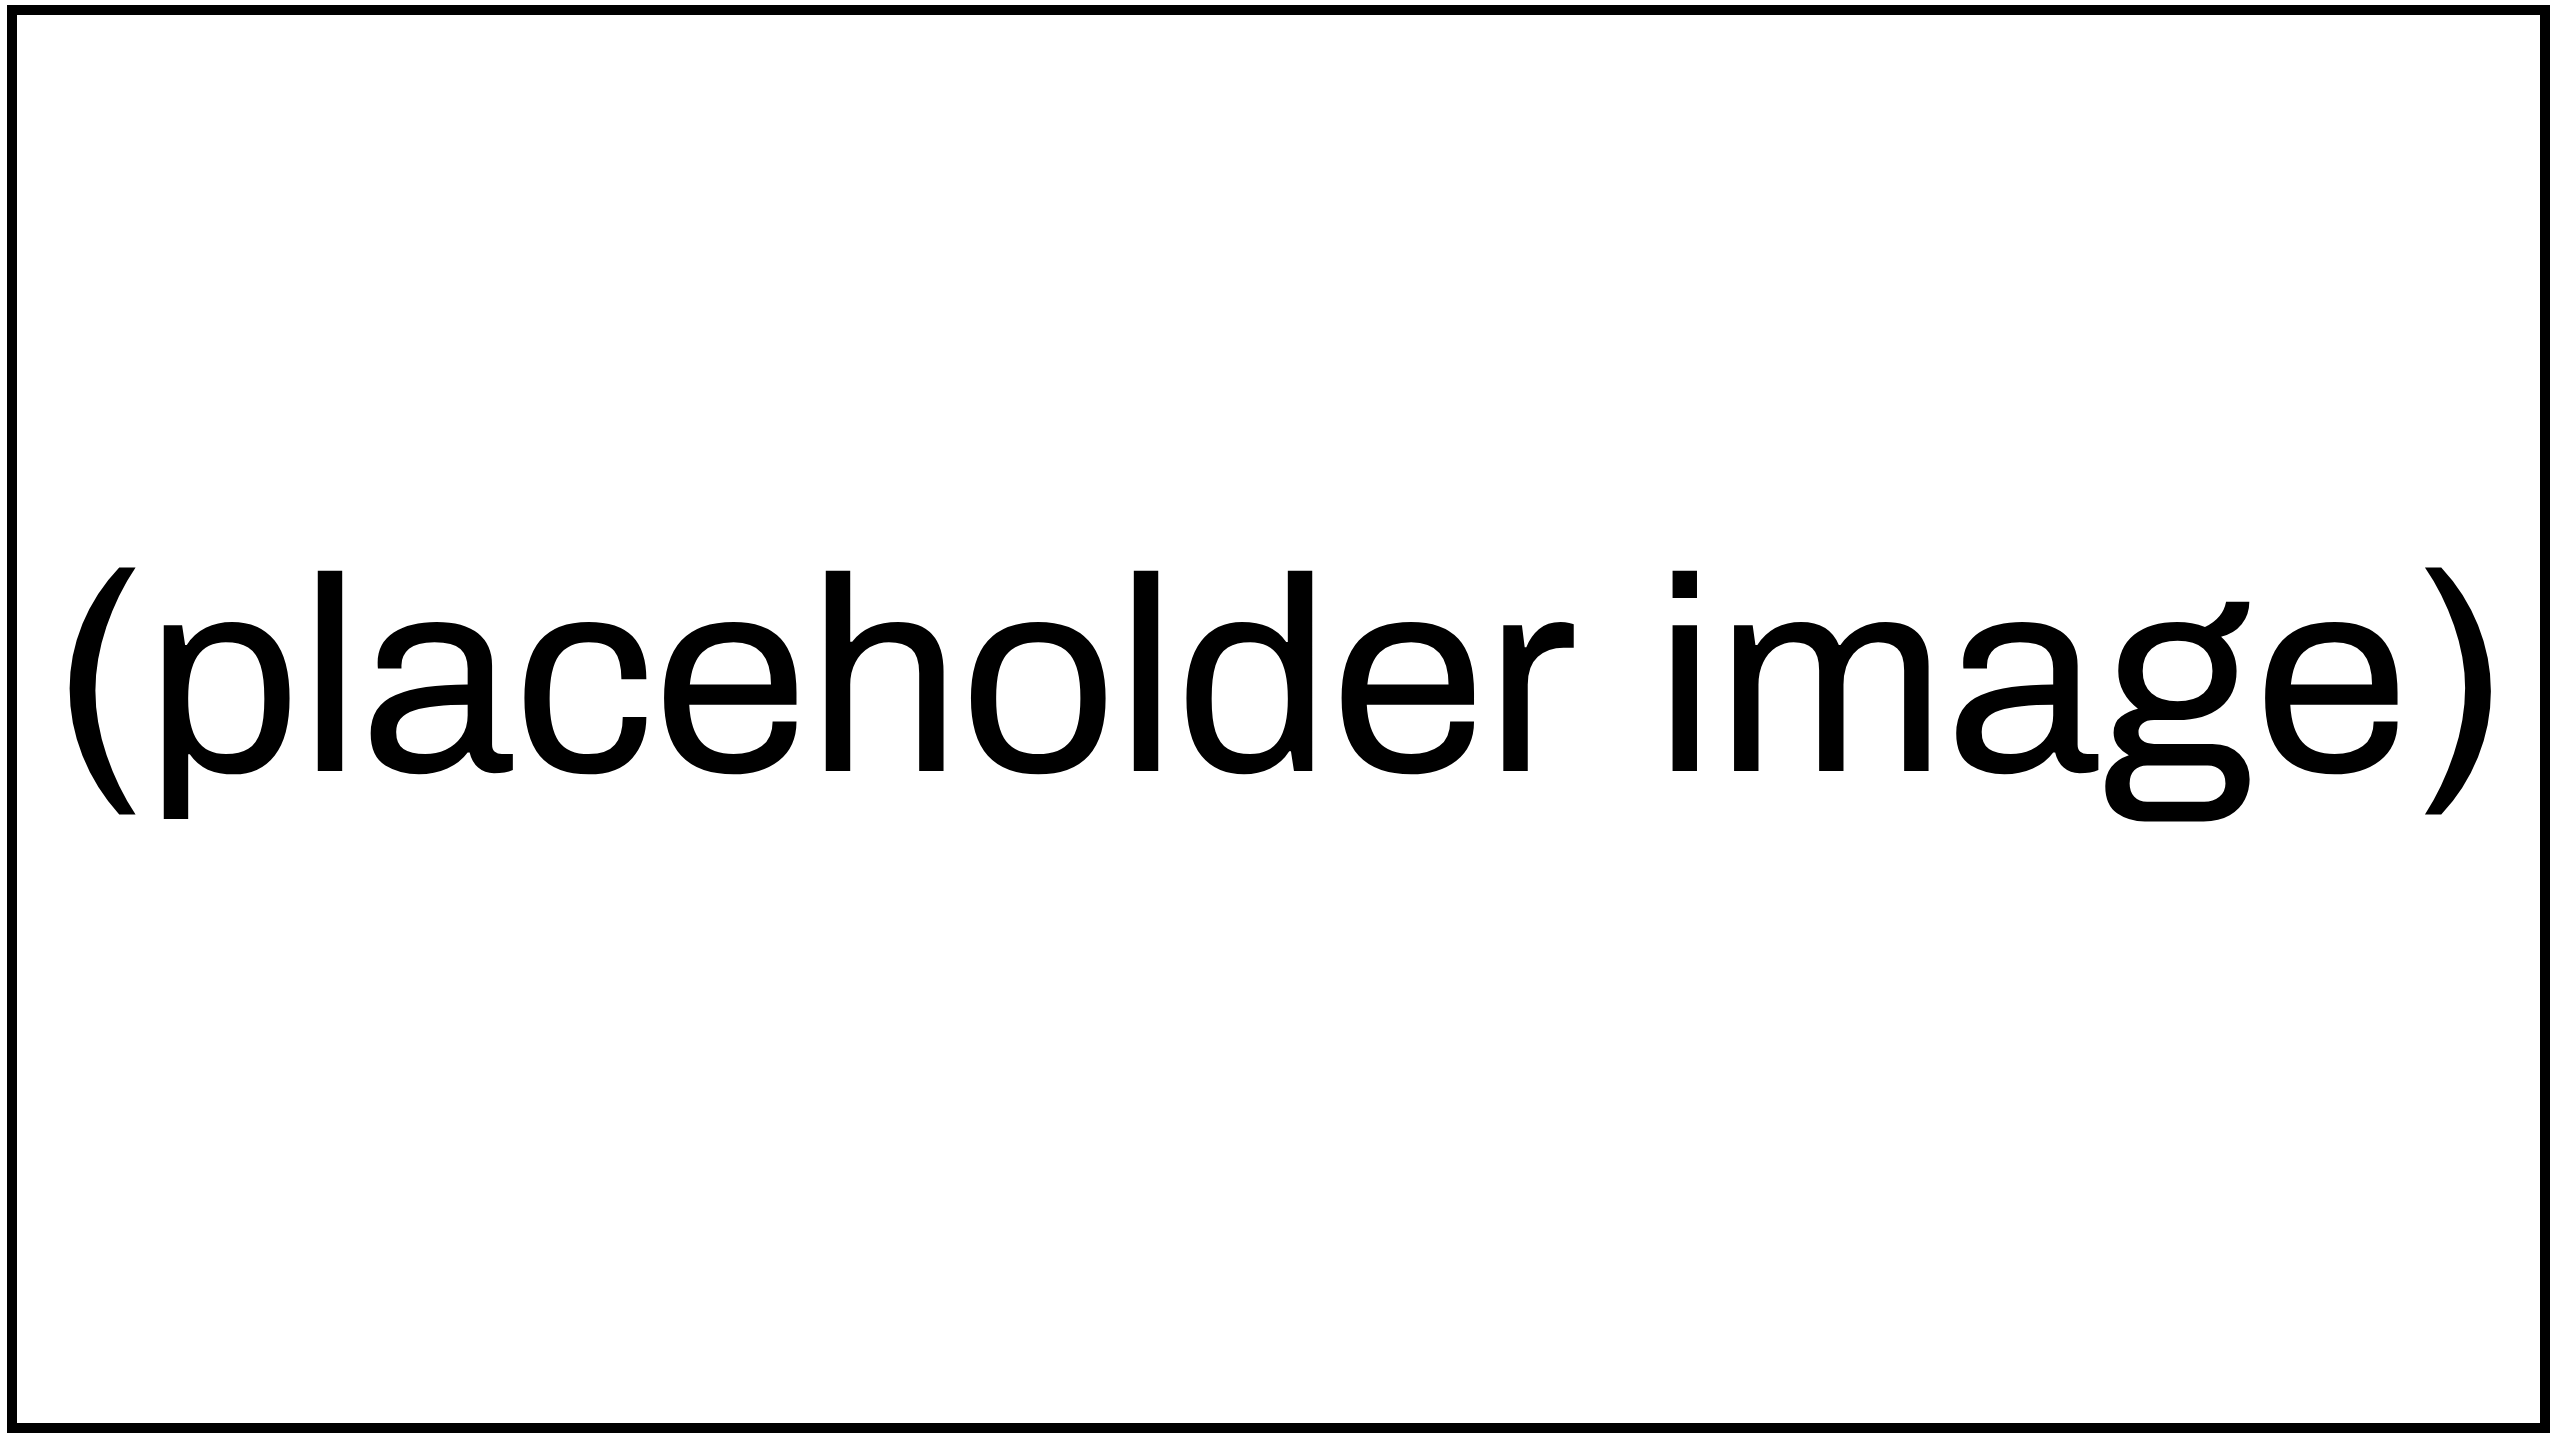
\includegraphics[width=0.8\textwidth]{figures/implementation/placeholder_image.png}
        \caption{System Architecture and Data Flow}
        \label{fig:implementation_system_architecture_and_data_flow}
    \end{figure}

\section{Entry Point and Command-Line Interface (CLI)}
\label{sec:entry_point_and_command_line_interface_cli}
This section describes the main entry point of \textbf{SMKIT}, the \texttt{smkit.py} script. It explains how \textbf{argparse} is used to manage command-line arguments and how the system operates based on user input.

\subsection{SMKIT Entry Point (\texttt{smkit.py})}
\label{subsec:smkit_entry_point_smkit_py}
The \texttt{smkit.py} script serves as the main entry point for \textbf{SMKIT}. This section explains the role of \textbf{argparse} in managing command-line arguments and how different options (e.g., \texttt{--module}, \texttt{--pages}, \texttt{--post\_type}, \texttt{--language}) determine the behavior of the system.

\subsection{Workflow Overview}
\label{subsec:workflow_overview}
This subsection provides a step-by-step overview of how \textbf{SMKIT} is used, from command-line input to content posting. It explains the flow of data through the system and how different modules work together to create and share content on social media platforms.

\section{Schema Management and Data Handling}
\label{sec:schema_management_and_data_handling}
This section discusses the various schemas used in \textbf{SMKIT} to manage and structure the data. The \texttt{PageInfo} and \texttt{NegapediaPageInfo} schemas play a key role in transforming raw data into usable content for social media posts.

\subsection{PageInfo Schema}
\label{subsec:pageinfo_schema}
The \texttt{PageInfo schema} is used for handling metadata from general websites, including fields such as title, description, and image URLs. This section describes the structure of the schema and its use in organizing data for social media posts.

\subsection{NegapediaPageInfo Schema}
\label{subsec:negapediapageinfo_schema}
The \texttt{NegapediaPageInfo schema} is used specifically for processing data from the Negapedia website. This schema contains additional fields tailored to Negapedia content, such as conflict and polemic awards, social jumps, and words that matter.

\section{Core Modules Implementation}
\label{sec:core_modules_implementation}
This section breaks down the implementation of the core modules in \textbf{SMKIT}. Each module is discussed in detail, including its responsibilities and how it contributes to the overall functionality of the system.

\subsection{Base Module}
\label{subsec:base_module}
The \textbf{Base Module} provides common functionality shared across all other modules in \textbf{SMKIT}. It includes initialization logic, error handling, logging, and other utilities necessary for the operation of the system.

\subsection{Generic Module}
\label{subsec:generic_module}
The \textbf{Generic Module} is responsible for processing web pages and extracting metadata (e.g., using \textbf{Open Graph} tags). This module can work with any website that implements \textbf{Open Graph} tags or similar structured data formats. It handles data extraction, transformation, and posting to social media platforms.

\subsection{Negapedia Module}
\label{subsec:negapedia_module}
The \textbf{Negapedia Module} is designed specifically to handle data from Negapedia. This section explains how the \texttt{NegapediaPageInfo} schema is used to structure and process Negapedia-specific data (e.g., conflict, polemic, social interaction metrics). The module processes this data and formats it for social media posting.

\section{Social Media Integration}
\label{sec:social_media_integration}
This section covers the integration with social media platforms like \textbf{Facebook} and \textbf{Twitter}. It explains how \textbf{SMKIT} interacts with their APIs to automate posting content and how the Web Connector module allows for the sharing of content via web pages.

\subsection{Facebook Connector}
\label{subsec:facebook_connector}
The \textbf{Facebook Connector} integrates \textbf{SMKIT} with Facebook’s Graph API to allow for seamless posting of content. This section covers the OAuth authentication process, rate limiting issues, and how posts are created and formatted to comply with Facebook's requirements.

\subsection{Twitter Connector}
\label{subsec:twitter_connector}
The \textbf{Twitter Connector} uses \texttt{Tweepy} to interact with the Twitter API, allowing for posting tweets. This section discusses the integration process, handling rate limits, and adapting content for Twitter's specific formatting requirements (e.g., tweet length, image attachments).

\subsection{Unified Social Media Posting}
\label{subsec:unified_social_media_posting}
This subsection explains how \textbf{SMKIT} can post content to multiple social media platforms (e.g., \textbf{Facebook} and \textbf{Twitter}) in a unified manner. It also discusses how the system abstracts the social media platform differences, making it easy to add future platforms.

\subsection{Web Connector and Content Sharing via Web Pages}
\label{subsec:web_connector_content_sharing}
In addition to posting on social media platforms, \textbf{SMKIT} can generate HTML web pages containing the same content shared on social media. This allows users to share content through a URL, providing an additional method of content distribution.

\section{Template Management and Customization}
\label{sec:template_management_and_customization}
Templates are an essential part of \textbf{SMKIT}, as they allow for dynamic content generation across different social media platforms and web pages. This section explains how templates are managed and how \textbf{SMKIT} customizes them based on user input.

\subsection{Template Overview}
\label{subsec:template_overview}
In this subsection, describe the role of templates in \textbf{SMKIT}. Explain how different templates are used for \textbf{Facebook}, \textbf{Twitter}, and web posts, and how the system chooses the appropriate template for each scenario.

\subsection{Template Customization and Data Insertion}
\label{subsec:template_customization_and_data_insertion}
This section explains how \textbf{SMKIT} dynamically populates templates with data (e.g., post titles, descriptions). It discusses how content from the \texttt{PageInfo} and \texttt{NegapediaPageInfo} schemas is inserted into the templates for social media posts.

\subsection{Web Connector and Web Page Generation}
\label{subsec:web_connector_and_web_page_generation}
In addition to posting content on social media platforms, \textbf{SMKIT} is also capable of generating HTML web pages that mirror the content shared on social media. The \textbf{Web Connector} module takes the content prepared for social media and converts it into HTML format, creating a web page that can be shared publicly.

The web pages generated by the Web Connector follow the same structure and content as the social media posts, ensuring consistency across platforms. The process involves dynamically populating HTML templates with the same data (e.g., titles, descriptions, images, etc.) that are used in the social media posts. This allows users to share content not only on social media platforms but also via a web URL.

The Web Connector allows SMKIT to:
\begin{itemize}
    \item \textbf{Generate HTML pages}: Create static HTML pages using predefined templates.
    \item \textbf{Consistency with Social Media Posts}: Ensure that the content shared on social media is identical to the web page content.
    \item \textbf{Customizable Templates}: Allow customization of the HTML templates to fit different design styles or specific content needs.
    \item \textbf{Easy Sharing}: Make it easy to share content on websites through URLs, providing an alternative to sharing only on social media.
\end{itemize}

\section{Utility Functions and Support Modules}
\label{sec:utility_functions_and_support_modules}
\textbf{SMKIT} relies on several utility functions and support modules to handle tasks like input validation, environment configuration, and logging. This section outlines the implementation of these supporting modules.

\subsection{Environment Management}
\label{subsec:Environment_management}
The \textbf{env\_management} module handles configuration settings, such as API keys and environment variables. This section discusses how the system securely manages sensitive information and loads configuration settings from environment files (e.g., \texttt{env.json}).

\subsection{Input Validation Management}
\label{subsec:input_validation_management}
This module ensures that user inputs (e.g., URLs, post types) are validated before being processed. It checks for required fields and formats, ensuring that only valid input is passed to the system.

\subsection{Image Management}
\label{subsec:image_management}
This section explains the \textbf{image\_management} module, which handles image retrieval, resizing, and preparation for posting. It ensures that images are correctly formatted according to the requirements of each social media platform.

\subsection{Logger Management}
\label{subsec:logger_management}
The \textbf{logger\_management} module ensures that \textbf{SMKIT} logs relevant system activities, including data extraction, errors, and performance metrics. This section explains how logging is integrated into the system for troubleshooting and monitoring.

\subsection{Plot Colors Management}
\label{subsec:plot_colors_management}
This utility manages color schemes used in visualizations, such as graphs representing conflict or social metrics. It ensures consistent and customizable color usage across the system.

\subsection{Translation Management}
\label{subsec:translation_management}
This section explains the \textbf{translation\_management} module, which handles language-specific templates and messages. It enables \textbf{SMKIT} to generate posts in multiple languages based on user input.

\section{Conclusion}
\label{sec:implementation_conclusion}
This section summarizes the key aspects of the \textbf{SMKIT} implementation, reflecting on the design choices and technical challenges. It provides a transition to the next chapter, which will discuss the \textbf{Results} of using \textbf{SMKIT} in real-world scenarios.
